\chapter{Tests und Experimente}
\label{cha:tests}

Im Kapitel Tests und Experimente werden unterschiedliche Hyperparameter-Konfigurationen auf ihre Auswirkungen getestet. Außerdem wird mit unterschiedlichen
Netzwerk-Architekturen die Performanz auf Geräten mit leistungsarmer Hardware gemessen.

\section{Auswirkungen der Hyperparameter}

Im Folgenden werden unterschiedliche Kombinationen der Gewichtungsparameter Content-Weight $ \alpha $, Style-Weight $ \beta $ und Total-Variation-Weight $ \gamma $ getestet. Dabei wird als Inhaltsbild  eine eigene Abbildung der HTW-Berlin benutzt. Als Stilbild wird das Kunstwerk The Starry Night des Künstlers Vincent Van Gogh und The Scream von Edvard Munch verwendet. Die generierten Bilder entsprechen einer Größe von 768 * 768 Pixel. Die restlichen Hyperparameter werden aus dem Kapitel Methodologie \ref{sec:method_neural_style_transfer} übernommen.

\pagebreak

\subsection{Experiment 1: Starry Night}

In diesem Experiment wird das Stilbild The Starry Night von Vincent Van Gogh verwendet.

\begin{figure}[H]
    \centering
    \begin{subfigure}[h]{0.20\textwidth}
        \centering
        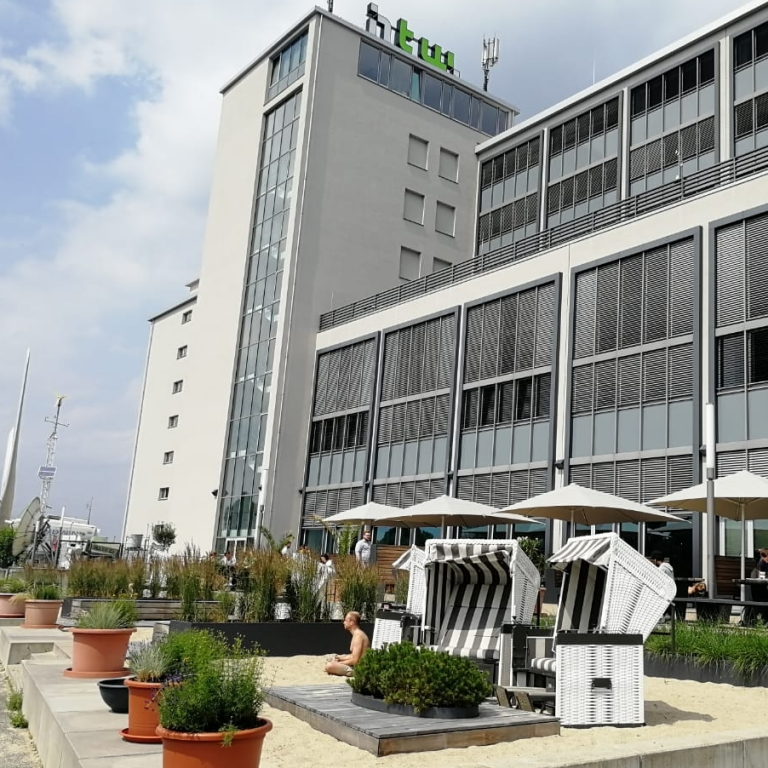
\includegraphics[width=\textwidth]{resources/content/content/htw-768x768.jpg}
    \end{subfigure}
    \begin{subfigure}[h]{0.20\textwidth}
        \centering
        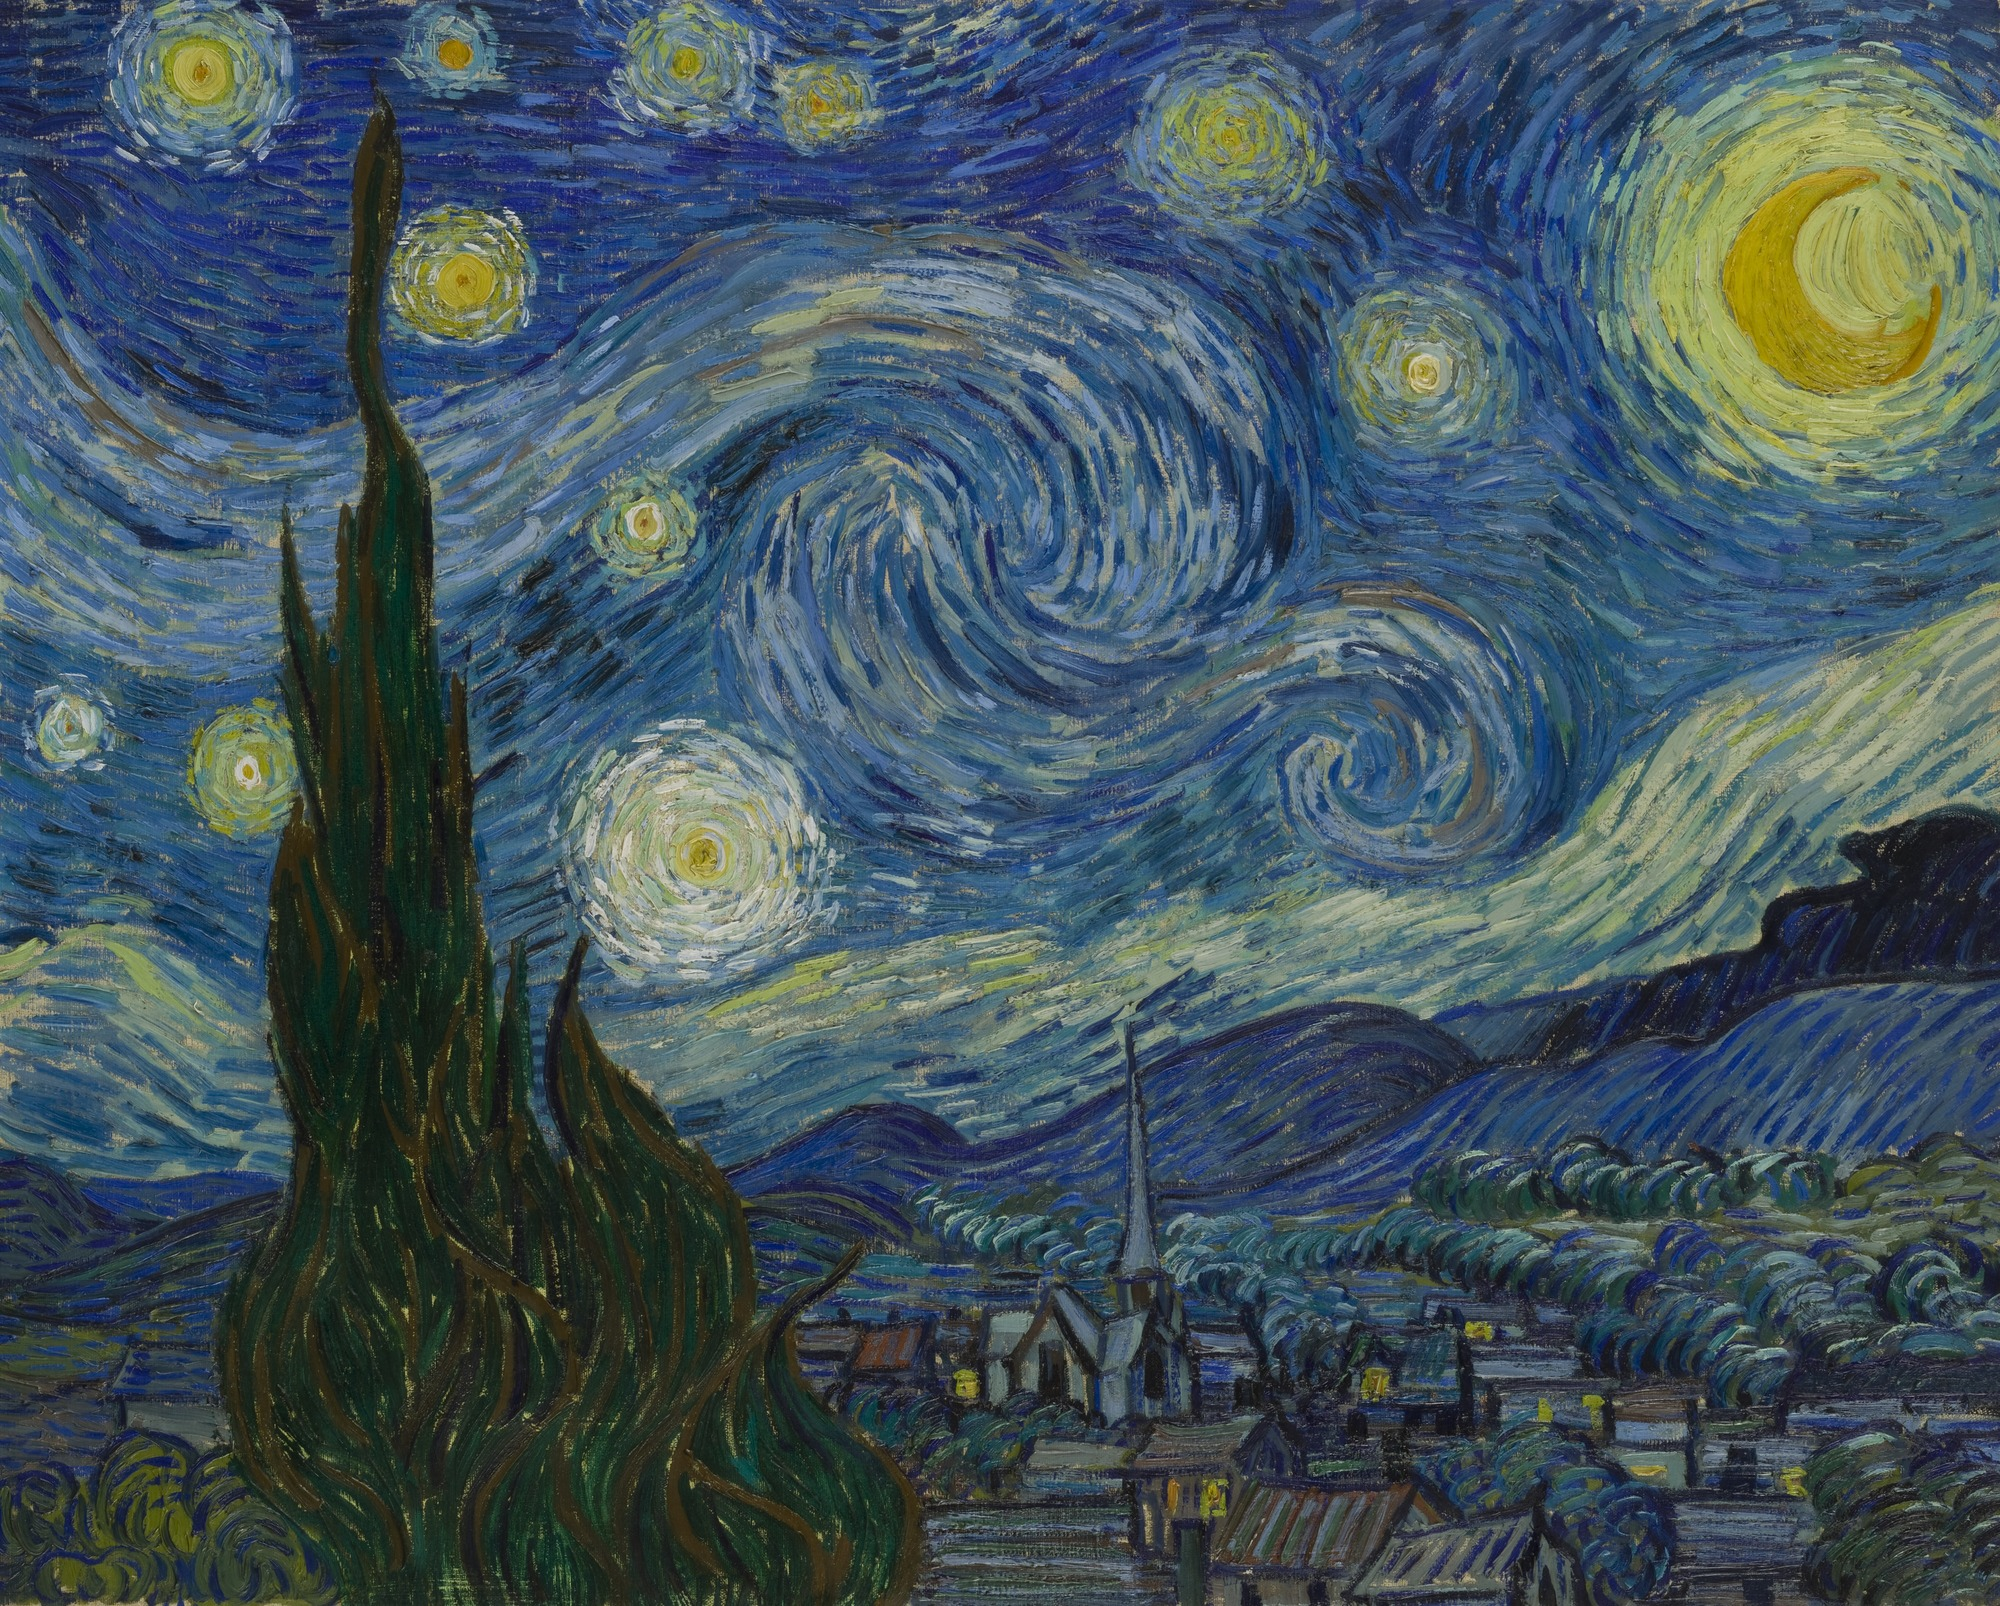
\includegraphics[width=\textwidth]{resources/content/style/starry_night.jpg}
    \end{subfigure}
    \caption{HTW kombiniert mit The Starry Night \cite{the_starry_night_img}}
\end{figure}

In der ersten Abbildungen werden die verschiedenen
Stilgewichtungen $ \beta = 10^{5} $, $ \beta = 10^{6} $, $ \beta = 10^{7} $, $ \beta = 10^{8} $ und $ \beta = 10^{9} $ für The Starry Night getestet.

\begin{figure}[H]
    \centering
    \begin{subfigure}[h]{0.15\textwidth}
        \centering
        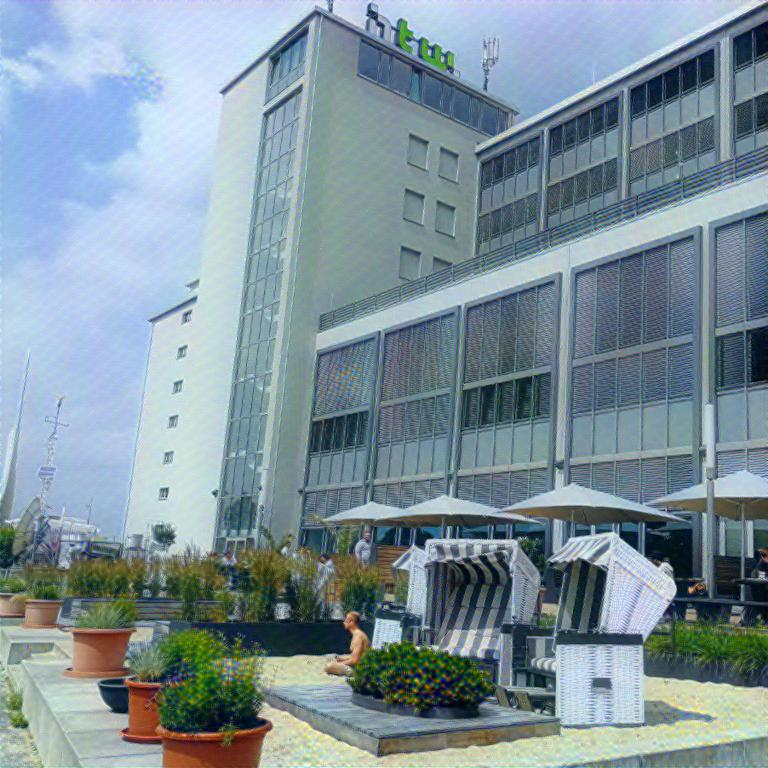
\includegraphics[width=\textwidth]{resources/content/experiments/a__starry_night__768x768__style-weight_1e+05__tv-weight_0e+00.jpg}
    \end{subfigure}
    \begin{subfigure}[h]{0.15\textwidth}
        \centering
        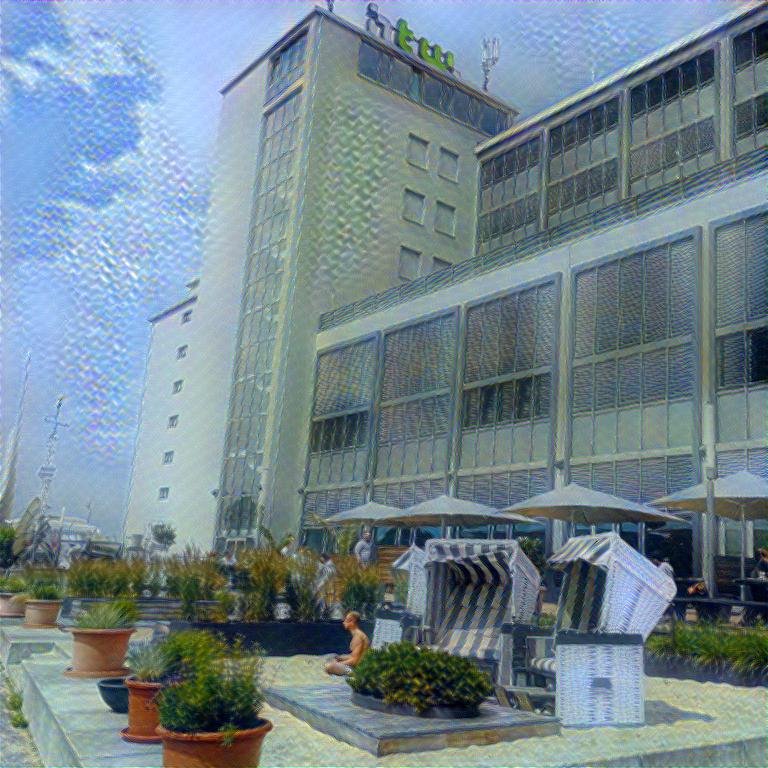
\includegraphics[width=\textwidth]{resources/content/experiments/a__starry_night__768x768__style-weight_1e+06__tv-weight_0e+00.jpg}
    \end{subfigure}
    \begin{subfigure}[h]{0.15\textwidth}
        \centering
        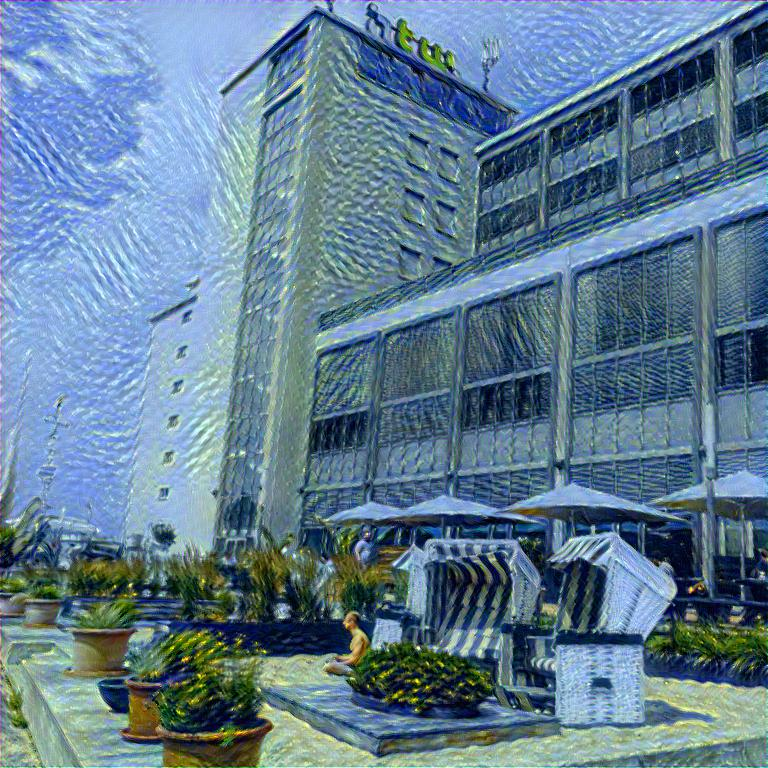
\includegraphics[width=\textwidth]{resources/content/experiments/a__starry_night__768x768__style-weight_1e+07__tv-weight_0e+00.jpg}
    \end{subfigure}
    \begin{subfigure}[h]{0.15\textwidth}
        \centering
        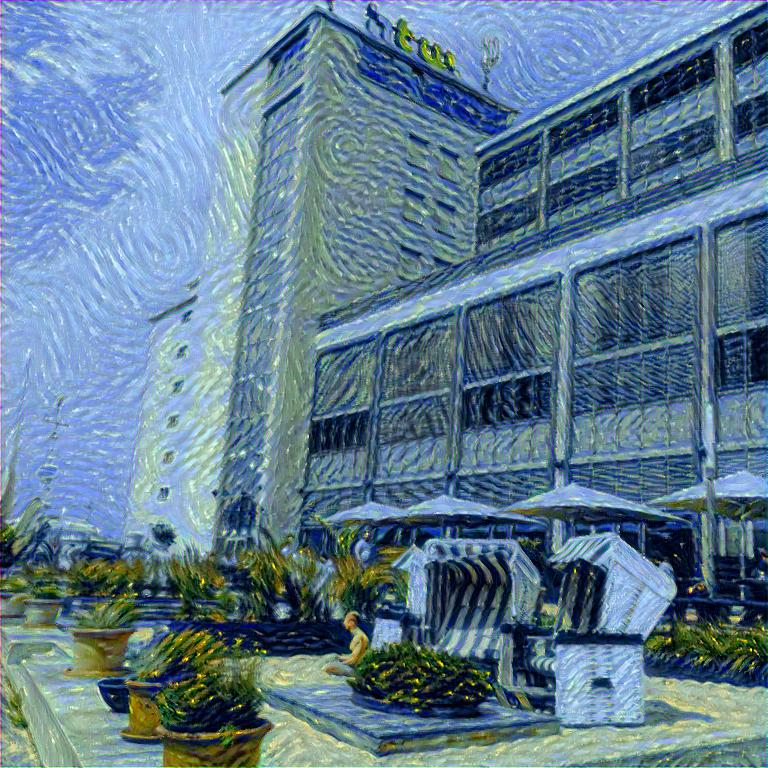
\includegraphics[width=\textwidth]{resources/content/experiments/a__starry_night__768x768__style-weight_1e+08__tv-weight_0e+00.jpg}
    \end{subfigure}
    \begin{subfigure}[h]{0.15\textwidth}
        \centering
        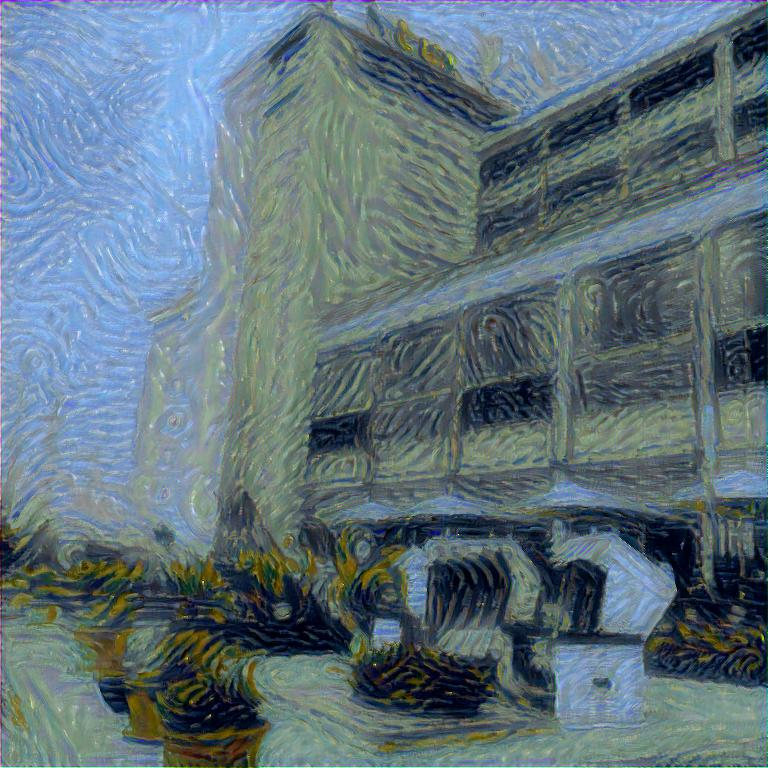
\includegraphics[width=\textwidth]{resources/content/experiments/a__starry_night__768x768__style-weight_1e+09__tv-weight_0e+00.jpg}
    \end{subfigure}
    \caption{The Starry Night mit $ \alpha = 1 $, $ \beta = 10^{5} - 10^{9} $, $ \gamma = 0 $}
\end{figure}

In der zweiten Abbildungen werden die verschiedenen Total-Variation-Gewichtungen $ \gamma = 10^{-7} $, $ \gamma = 10^{-6} $, $ \gamma = 10^{-5} $, $ \gamma = 10^{-4} $ und $ \gamma = 10^{-3} $  für Starry Night getestet.

\begin{figure}[H]
    \centering
    \begin{subfigure}[h]{0.15\textwidth}
        \centering
        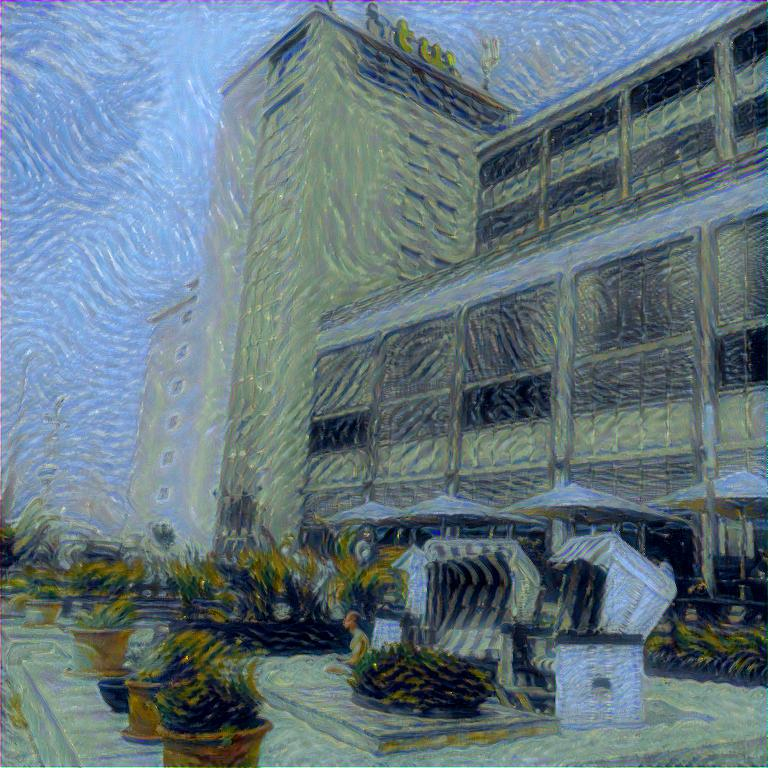
\includegraphics[width=\textwidth]{resources/content/experiments/b__starry_night__768x768__style-weight_1e+08__tv-weight_1e-07.jpg}
    \end{subfigure}
    \begin{subfigure}[h]{0.15\textwidth}
        \centering
        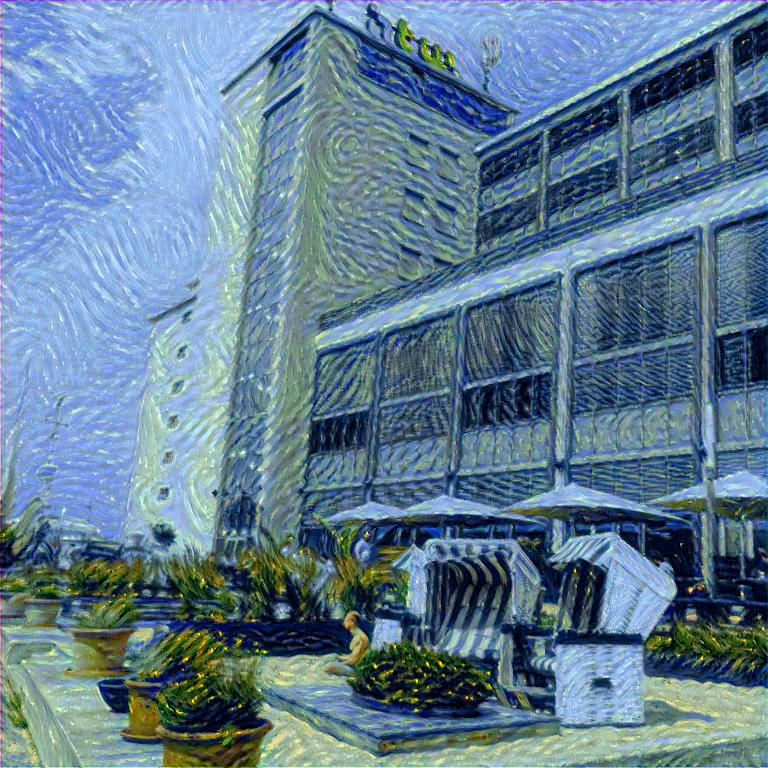
\includegraphics[width=\textwidth]{resources/content/experiments/b__starry_night__768x768__style-weight_1e+08__tv-weight_1e-06.jpg}
    \end{subfigure}
    \begin{subfigure}[h]{0.15\textwidth}
        \centering
        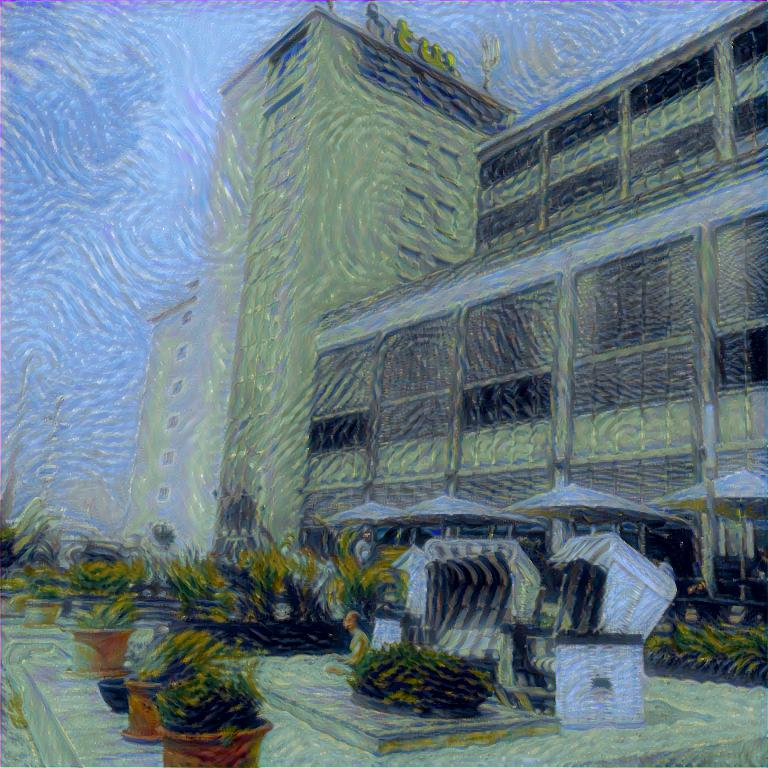
\includegraphics[width=\textwidth]{resources/content/experiments/b__starry_night__768x768__style-weight_1e+08__tv-weight_1e-05.jpg}
    \end{subfigure}
    \begin{subfigure}[h]{0.15\textwidth}
        \centering
        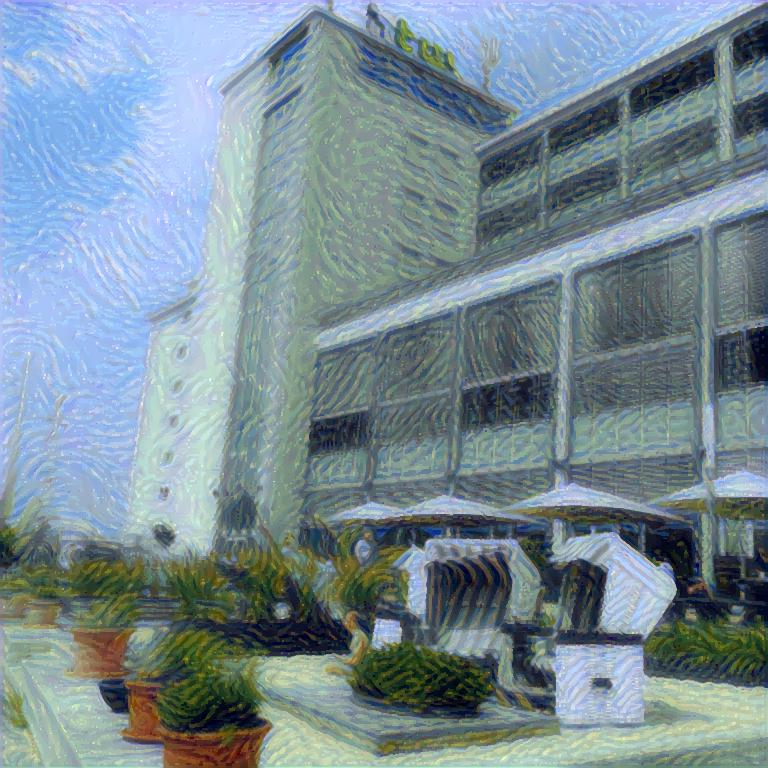
\includegraphics[width=\textwidth]{resources/content/experiments/b__starry_night__768x768__style-weight_1e+08__tv-weight_1e-04.jpg}
    \end{subfigure}
    \begin{subfigure}[h]{0.15\textwidth}
        \centering
        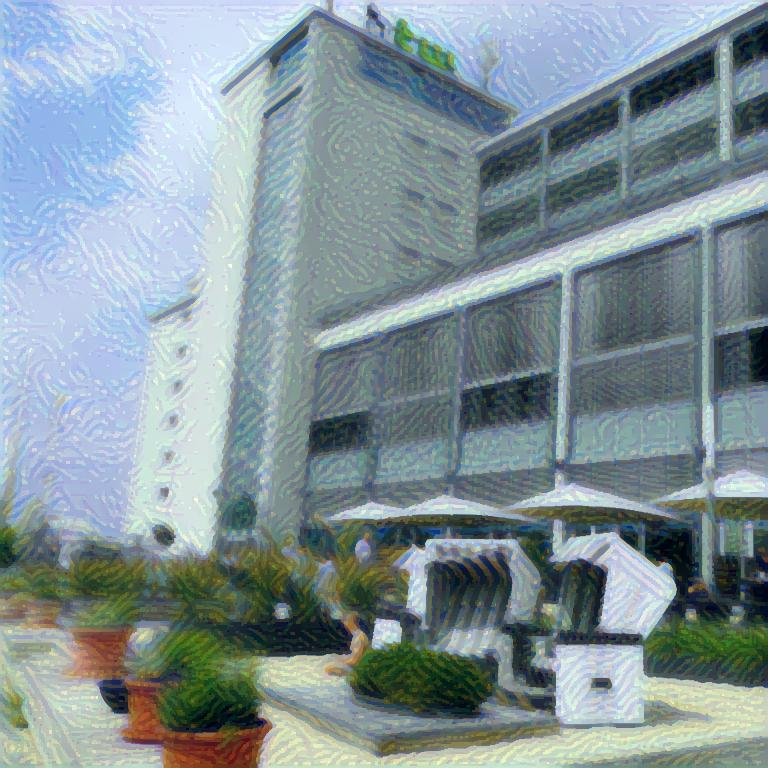
\includegraphics[width=\textwidth]{resources/content/experiments/b__starry_night__768x768__style-weight_1e+08__tv-weight_1e-03.jpg}
    \end{subfigure}
    \caption{Starry Night mit $ \alpha = 1 $, $ \beta = 10^{8} $, $ \gamma = 10^{-7} - 10^{-3} $}
\end{figure}

\pagebreak

\subsection{Experiment 2: The Scream}

\begin{figure}[H]
    \centering
    \begin{subfigure}[h]{0.20\textwidth}
        \centering
        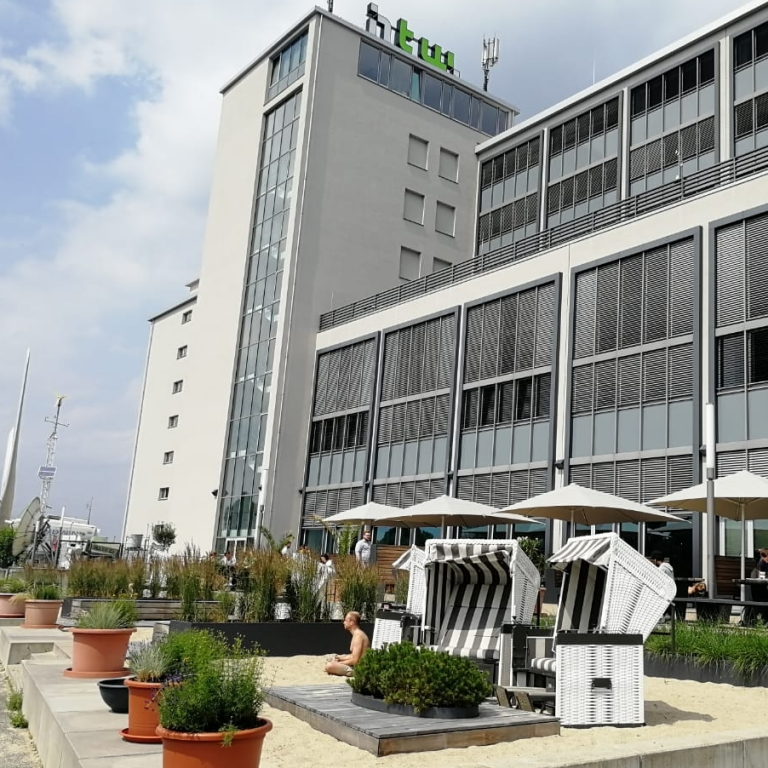
\includegraphics[width=\textwidth]{resources/content/content/htw-768x768.jpg}
    \end{subfigure}
    \begin{subfigure}[h]{0.20\textwidth}
        \centering
        \includegraphics[width=\textwidth]{resources/content/style/the_scream.jpg}
    \end{subfigure}
    \caption{HTW kombiniert mit The Scream \cite{the_scream_img}}
\end{figure}


In der ersten Abbildungen werden verschiedene die verschiedenen  \\
Stilgewichtungen $ \beta = 10^{5} $, $ \beta = 10^{6} $, $ \beta = 10^{7} $, $ \beta = 10^{8} $ und $ \beta = 10^{9} $ für The Scream getestet.

\begin{figure}[H]
    \centering
    \begin{subfigure}[h]{0.15\textwidth}
        \centering
        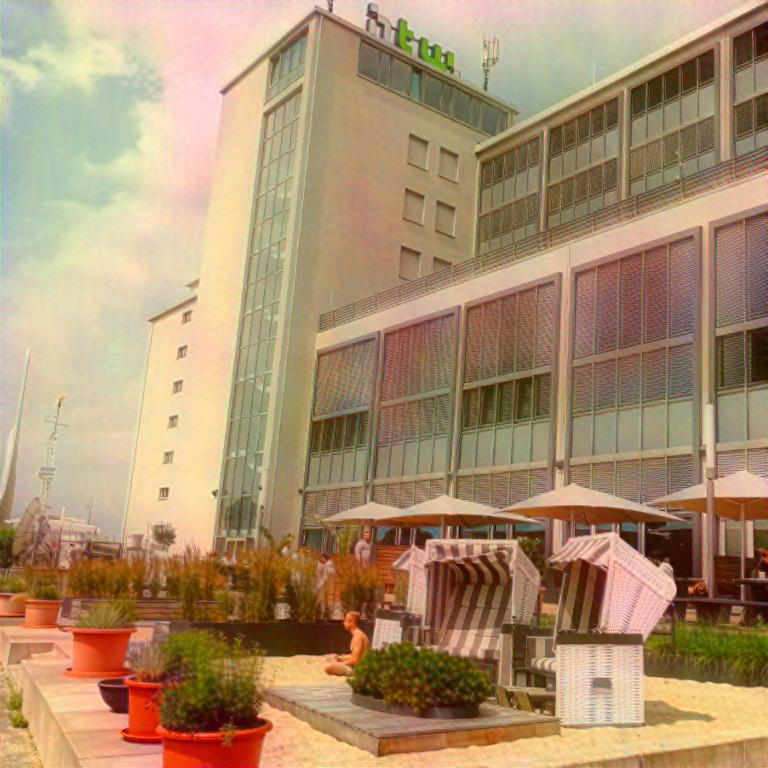
\includegraphics[width=\textwidth]{resources/content/experiments/a__the_scream__768x768__style-weight_1e+05__tv-weight_0e+00.jpg}
    \end{subfigure}
    \begin{subfigure}[h]{0.15\textwidth}
        \centering
        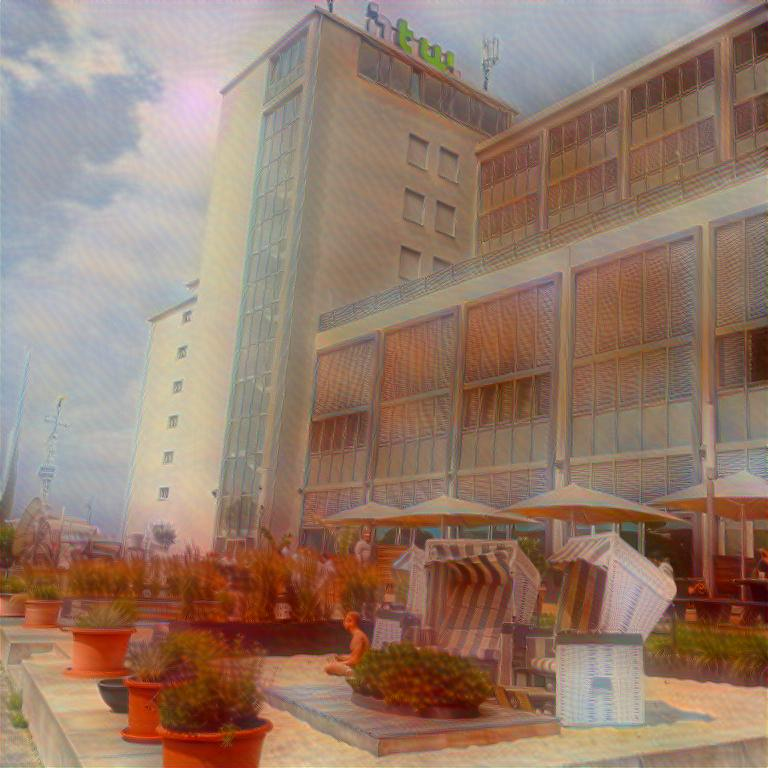
\includegraphics[width=\textwidth]{resources/content/experiments/a__the_scream__768x768__style-weight_1e+06__tv-weight_0e+00.jpg}
    \end{subfigure}
    \begin{subfigure}[h]{0.15\textwidth}
        \centering
        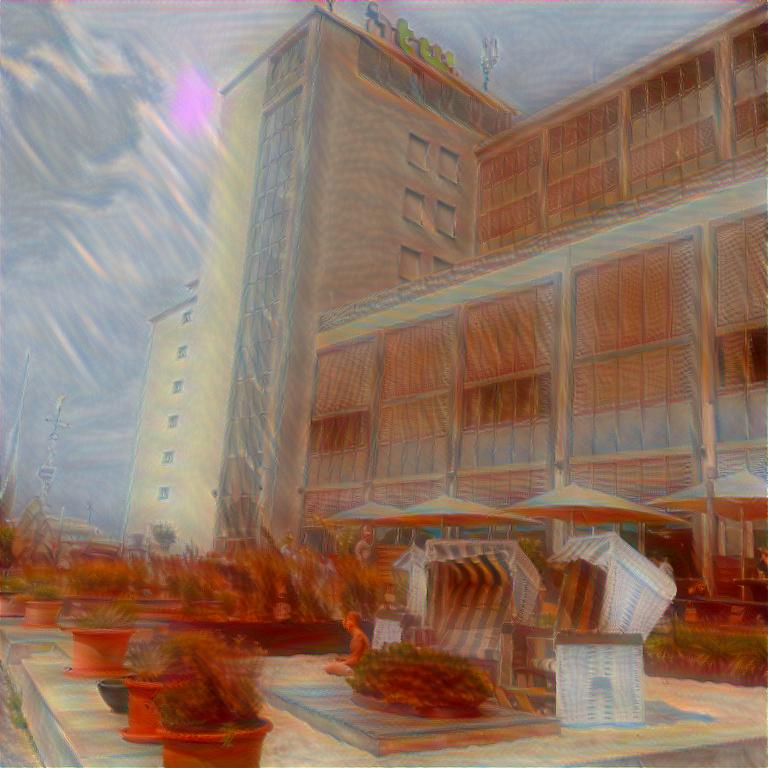
\includegraphics[width=\textwidth]{resources/content/experiments/a__the_scream__768x768__style-weight_1e+07__tv-weight_0e+00.jpg}
    \end{subfigure}
    \begin{subfigure}[h]{0.15\textwidth}
        \centering
        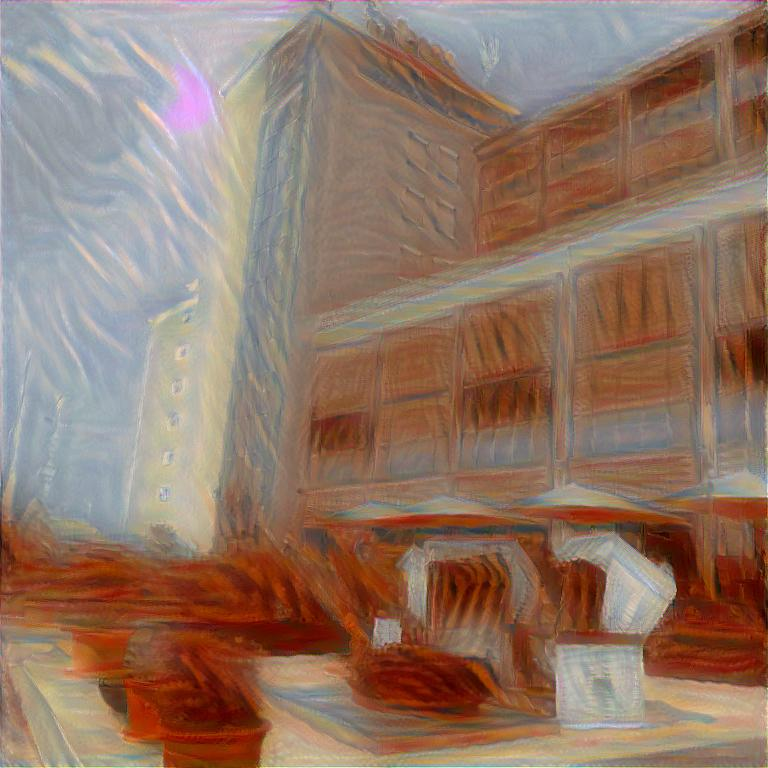
\includegraphics[width=\textwidth]{resources/content/experiments/a__the_scream__768x768__style-weight_1e+08__tv-weight_0e+00.jpg}
    \end{subfigure}
    \begin{subfigure}[h]{0.15\textwidth}
        \centering
        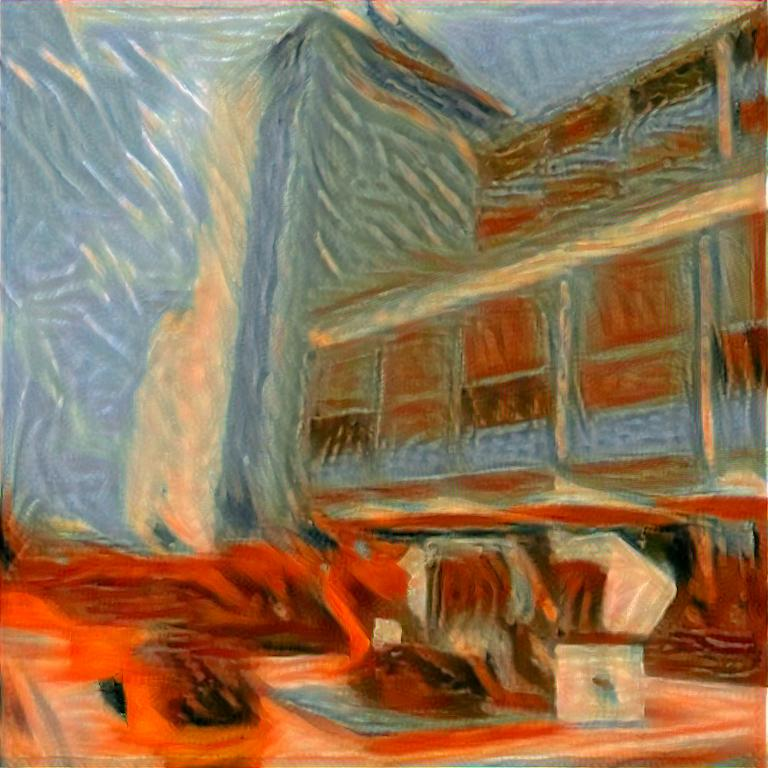
\includegraphics[width=\textwidth]{resources/content/experiments/a__the_scream__768x768__style-weight_1e+09__tv-weight_0e+00.jpg}
    \end{subfigure}
    \caption{The Scream mit $ \alpha = 1 $, $ \beta = 10^{5} - 10^{9} $, $ \gamma = 0 $}
\end{figure}

In der zweiten Abbildungen werden verschiedene die verschiedenen Total-Variation-Gewichtungen $ \gamma = 10^{-7} $, $ \gamma = 10^{-6} $, $ \gamma = 10^{-5} $, $ \gamma = 10^{-4} $ und $ \gamma = 10^{-3} $ für The Scream getestet.

\begin{figure}[H]
    \centering
    \begin{subfigure}[h]{0.15\textwidth}
        \centering
        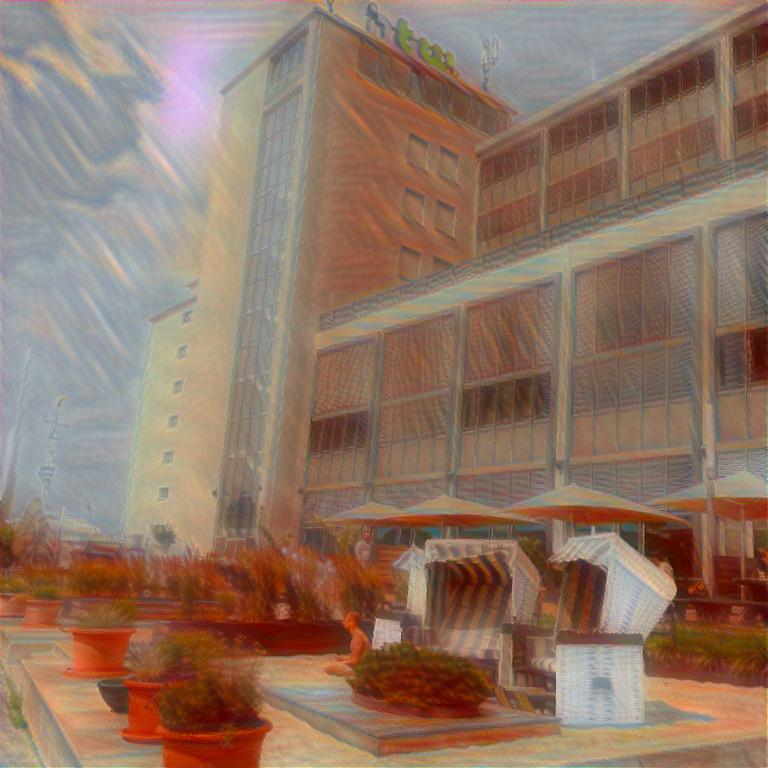
\includegraphics[width=\textwidth]{resources/content/experiments/b__the_scream__768x768__style-weight_1e+07__tv-weight_1e-07.jpg}
    \end{subfigure}
    \begin{subfigure}[h]{0.15\textwidth}
        \centering
        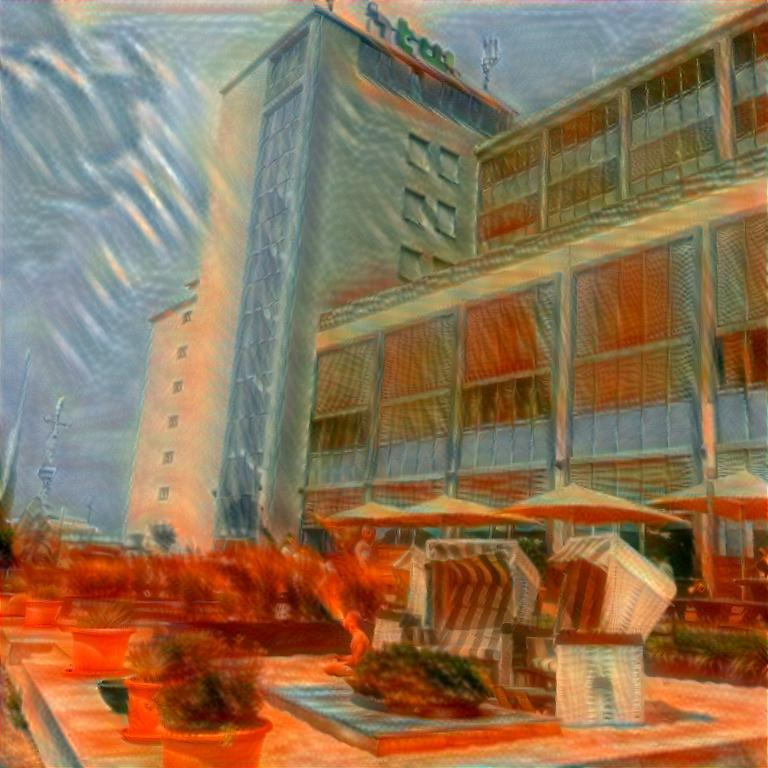
\includegraphics[width=\textwidth]{resources/content/experiments/b__the_scream__768x768__style-weight_1e+07__tv-weight_1e-06.jpg}
    \end{subfigure}
    \begin{subfigure}[h]{0.15\textwidth}
        \centering
        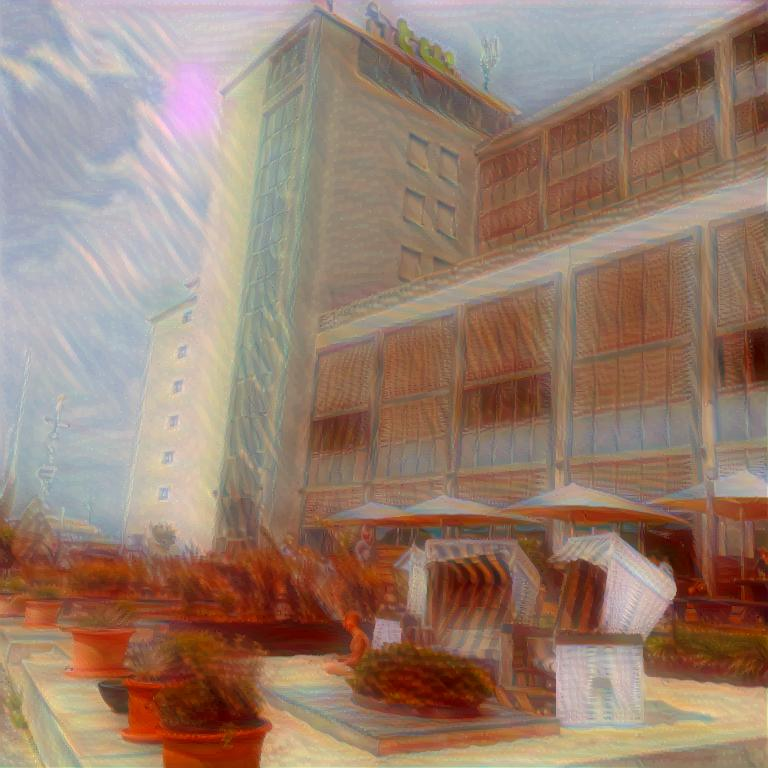
\includegraphics[width=\textwidth]{resources/content/experiments/b__the_scream__768x768__style-weight_1e+07__tv-weight_1e-05.jpg}
    \end{subfigure}
    \begin{subfigure}[h]{0.15\textwidth}
        \centering
        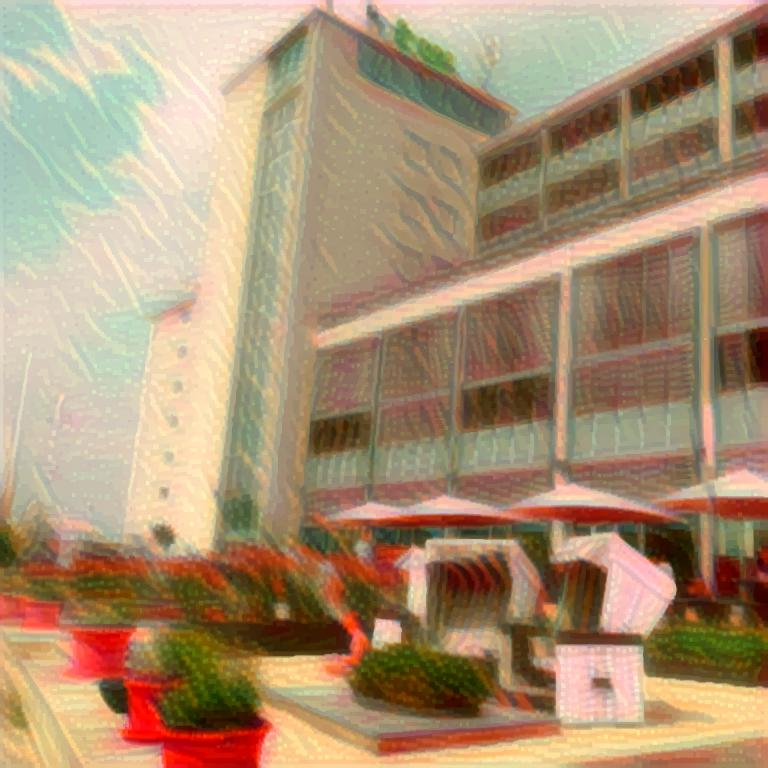
\includegraphics[width=\textwidth]{resources/content/experiments/b__the_scream__768x768__style-weight_1e+07__tv-weight_1e-04.jpg}
    \end{subfigure}
    \begin{subfigure}[h]{0.15\textwidth}
        \centering
        
\includegraphics[width=\textwidth]{resources/content/experiments/b__the_scream__768x768__style-weight_1e+07__tv-weight_1e-03.jpg}
    \end{subfigure}
    \caption{The Scream mit $ \alpha = 1 $, $ \beta = 10^{7} $, $ \gamma = 10^{-7} - 10^{-3} $}
\end{figure}

\pagebreak

\subsection{Interpretation der Ergebnisse}

Wie beiden Tests zu sehen ist, werden die Muster mit zunehmendem Style-Weight $ \beta $ auf dem Ausgangsbild immer stärker generierten. Mit $ b = 10^{5} $ sind bei beiden Stilen die Muster des Gemäldes kaum noch zu erkennen. Lediglich wird das Ausgangsbild den Farben des Stilbildes angepasst. Ein optisch ansprechender Effekt ergibt sich bei beiden Stilen ab $ \beta = 10^{7} $. 

Mit zunehmendem Total-Variation-Weight $ \gamma $ fließen die Farben mehr ineinander und das Ausgangsbild wird verschommener. Das ist besodners gut zu sehen bei The Starry Night mit $ \gamma = 10^{-3} $ und \text{The Scream} mit $ \gamma = 10^{-4} $. Für The Scream ist eine Gewichtung von $ \gamma = 10^{-3} $ bereits zu hoch gewählt. Das Ausgangsbild entwickelt sich zu einem grauen Rauschen.


\section{Auswirkungen der Netzwerkarchitekturen}

Im diesem Experiment wurden drei unterschiedlichen Bildgrößen auf unterschiedlichen Geräten auf Durchführbarkeit und Performanz getestet.
Gemessen wird die Berechnungsgeschwindigkeit beim Forward-Pass durch das Netzwerk. Ein bereits erster Indikator für die Performanz eines Neuronalen Netzwerks ist die Anzahl der lernbaren Parameter, die bei der Trainingsphase optimiert werden. Erstellt wurden neun unterschiedliche Netzwerke mit dem Kunstwerk The Starry Night mit unterschiedlichen Kombinationen für $ m $ und $ s $. 

\begin{table}[H]
    \centering
    \begin{tabular}{ |c|c|c|c| }
        \hline
        \textbf{Name} & \textbf{Bottleneck Size $ s $} & \textbf{Multiplkator $ m $} & \textbf{Anzahl lernbarer Parameter} \\ \hline
        Netzwerk 1 & 5 & 32 & 2.006.931 \\ \hline
        Netzwerk 2 & 5 & 16 & 506.835 \\ \hline
        Netzwerk 3 & 5 & 8  & 129.267 \\ \hline

        Netzwerk 4 & 4 & 32 & 1.711.250 \\ \hline
        Netzwerk 5 & 4 & 16 & 432.722 \\ \hline
        Netzwerk 6 & 4 & 8  & 110.642 \\ \hline

        Netzwerk 7 & 3 & 32 & 1.415.569 \\ \hline
        Netzwerk 8 & 3 & 16 & 358.609 \\ \hline
        Netzwerk 9 & 3 & 8  & 92.017 \\ \hline
    \end{tabular}
    \caption{Unterschiedliche Netzwerkgrößen und ihre Parameter}
    \label{tab:networks}
\end{table}

Bei der Berechnung des Forward-Pass macht es einen Unterschied ob sie  auf dem CPU oder dem GPU eines Geräts durchgeführt wird. Neuronale Netzwerke können auf einer GPU schneller als auf einem CPU berechnet werden. Das liegt daran, dass eine GPU besonders auf die Berechnung von Matrix-Operationen (wie Sie auch bei grafischen Anwendungen verwendet werden) spezialisiert ist.

Die Daten werden beim Einsatz des GPUs in den Grafikspeicher geladen. Bei der Berechnung über den CPU wird der Arbeitsspeicher (RAM) des Geräts verwendet. Der RAM kann über die Verwendung einer Auslagerungsdatei (SWAP-Datei) virtuell erweitert werden. Somit kann verhindert werden das es zu Fehlern wegen unzureichendem Arbeitsspeicher kommt.

\begin{table}[H]
    \centering
    \begin{tabular}{ |c|c| }
        \hline
        Prozessor       & Intel Core i7-6700HQ \\ \hline
        Grafikkarte     & NVIDIA® GeForce™ GTX 960M (2GB GDDR5) \\ \hline
        Arbeitsspeicher & 16GB DDR4  \\ \hline
        Festplatte      & 512GB SSD \\ \hline
    \end{tabular}
    \caption{Spezifikation: Dell XPS 15 9550}
    \label{tab:xps15}
\end{table}

\begin{table}[H]
    \centering
    \begin{tabular}{ |c|c| }
        \hline
        Prozessor       & Quad-Core ARM®Cortex®-A57 MPCore \\ \hline
        Grafikkarte     & 256-core NVIDIA Maxwell™ GPU \\ \hline
        Arbeitsspeicher & 4GB 64-bit LPDDR4  \\ \hline
        Festplatte      & 16GB eMMC 5.1 \\ \hline
    \end{tabular}
    \caption{Spezifikation: Jetson TX1}
    \label{tab:jetson_tx1}
\end{table}


Abschließend wurden die unterschiedlichen Netzwerkearchitekturen auf ihre Performanz getestet. Tests die wegen unzureichendem Arbeitsspeicher oder Grafikspeicher fehlschlagen sind, wurden als \textcolor{danger}{nicht durchführbar} gekennzeichnet. Um die Tests durchzuführen wurden Bilder der Größen 1920 * 1080 Pixel, 1024 * 786 Pixel und 640 * 480 Pixel jeweils 10 mal mit jedem Netzwerk berechnet, die Berechnugnsgeschwindigkeit gemessen, und das arithmische Mittel der 10 Durchläufe gebildet. Die Ergebnisse sind in den Anlagen \ref{tab:1920x1080}, \ref{tab:1024x768} und \ref{tab:640x480} angefügt.

\subsection{Interpretation der Ergebnisse}

Alle Netzwerke wurden mit einer Batch-Size von $ 24 $, Bildgrößen von 224 * 224 Pixel und einer Learning-Rate von $ 10^{-3} $ trainiert. Es wurden 4 Epochen der Trainingsdaten aus dem Jahr 2017 des COCO-Datensatzes verwendet, welche $ 118287 $ Bilder enthalten. Insgesamt wurden die Modelle mit $ 473148 $ Bildern trainiert. Dabei dauerte die Trainingszeit auf einem Server mit einem GeForce GTX 1080 Ti GPU pro Modell zwischen 3 und 6 Stunden.

Beim Training fiel auf das die generierten Bilder großflächige, schwarze oder weiße Artefakte enthielten. Ein Austausch der finalen Aktivierungsfunktion HardTanH, vgl. \ref{sec:hardtanh}, mit der Sigmoid-Aktivierungsfunktion, vgl. \ref{sec:sigmoid}, konnte das Problem lösen.

Auffällig bei den Messungen ist das der Parameter $ m $, welche die Anzahl der Channels im Netzwerk beeinflusst, bei Berechnungen auf dem CPU einen größere Performanzverbesserung bietet als der Parameter $ s $. Bei Berechnungen mit einem GPU ist der Parameter $ s $, Anzahl der ResidualBlocks weit aus relatanter für die Berechnugnsgeschwindigkeit des Netzwerks. Bei den Netzwerken 7, 8 und 9 spielt der Paramter $ m $ bei der Benutzung eines GPU fast garkeine Rolle mehr. Die Berechnung der Netzwerke mit Full HD Bildern war jedoch mit keinem der Netzwerke auf dem GPU möglich.

In der folgenden Abbildung ist zu sehen das alle Netzwerkarchitekturen, nach Austausch der finalen Aktivierungsfunktion, gleichermaßen in der Lagen waren den Stil von The Starry Night zu extrahieren.
Alle gelernten Muster sind zwar geringfügig unterschiedlich, jedoch optisch gleichermaßen ansprechend und dem Stil des Bildes The Starry Night ähnlich.

\begin{figure}[H]
    \centering
    \begin{subfigure}[h]{0.15\textwidth}
        \centering
        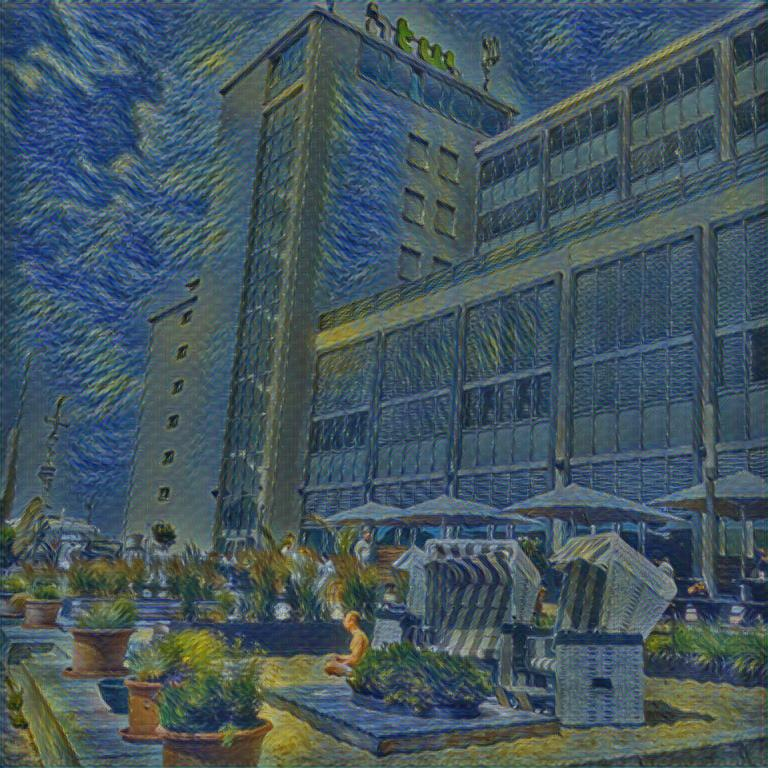
\includegraphics[width=\textwidth]{resources/content/experiments/net1.jpg}
    \end{subfigure}
    \begin{subfigure}[h]{0.15\textwidth}
        \centering
        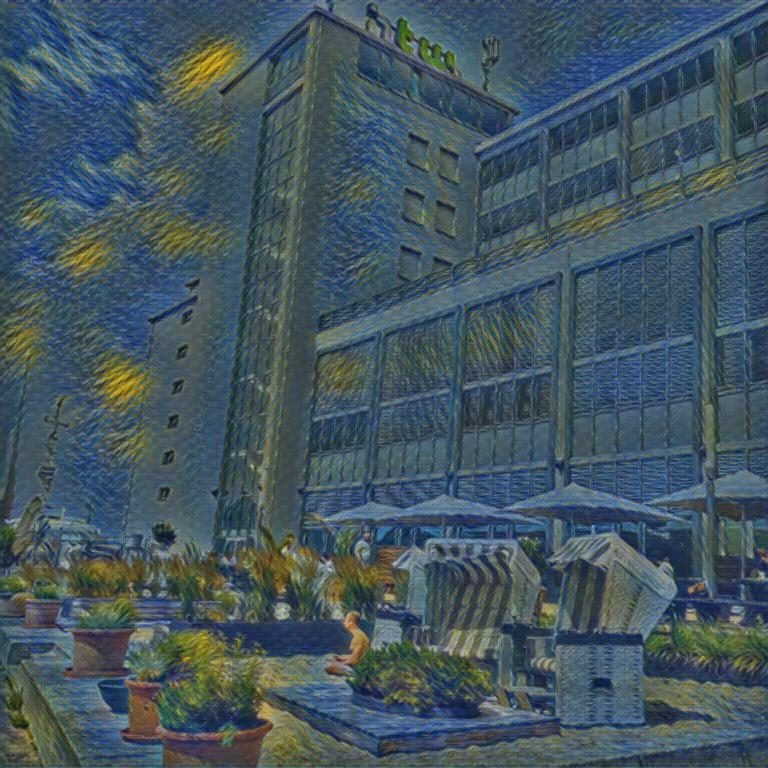
\includegraphics[width=\textwidth]{resources/content/experiments/net2.jpg}
    \end{subfigure}
    \begin{subfigure}[h]{0.15\textwidth}
        \centering
        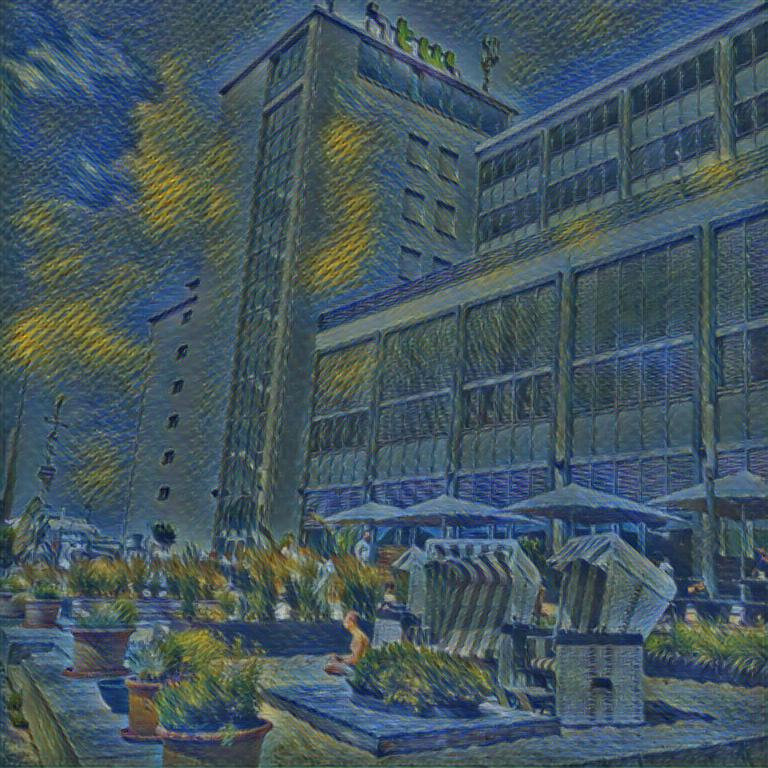
\includegraphics[width=\textwidth]{resources/content/experiments/net3.jpg}
    \end{subfigure} \\

    \begin{subfigure}[h]{0.15\textwidth}
        \centering
        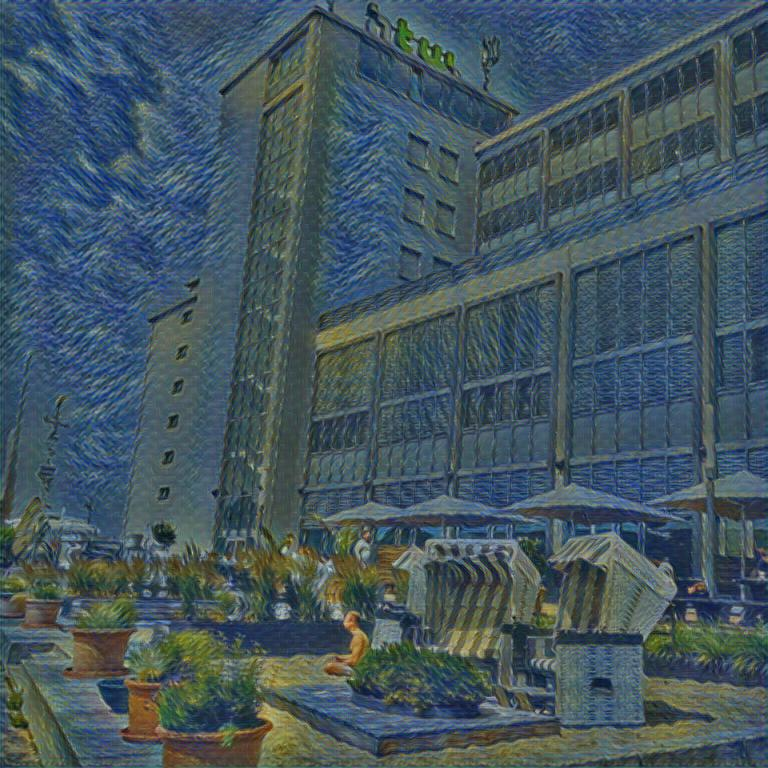
\includegraphics[width=\textwidth]{resources/content/experiments/net4.jpg}
    \end{subfigure}
    \begin{subfigure}[h]{0.15\textwidth}
        \centering
        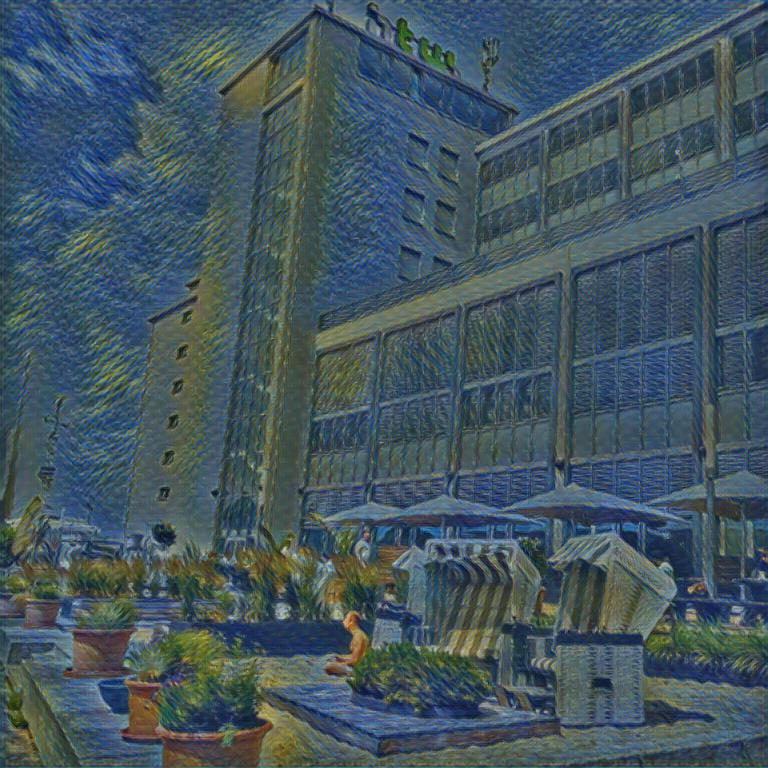
\includegraphics[width=\textwidth]{resources/content/experiments/net5.jpg}
    \end{subfigure}
    \begin{subfigure}[h]{0.15\textwidth}
        \centering
        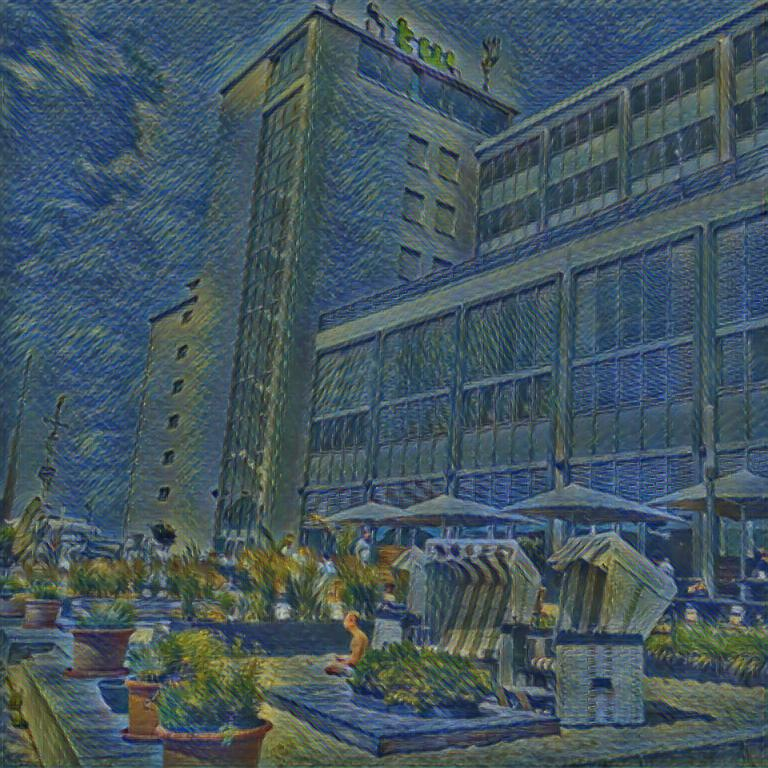
\includegraphics[width=\textwidth]{resources/content/experiments/net6.jpg}
    \end{subfigure} \\
    
    \begin{subfigure}[h]{0.15\textwidth}
        \centering
        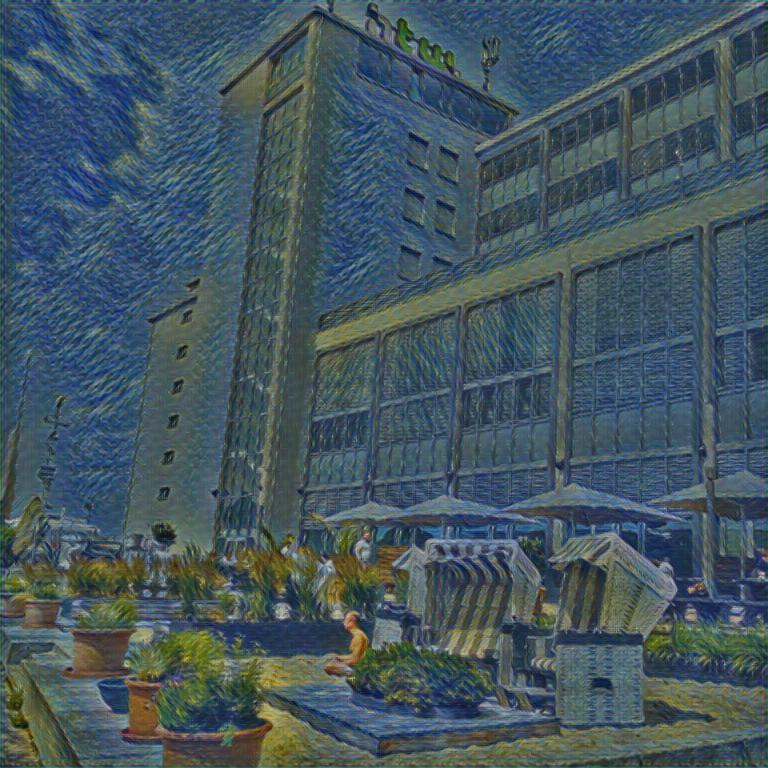
\includegraphics[width=\textwidth]{resources/content/experiments/net7.jpg}
    \end{subfigure}
    \begin{subfigure}[h]{0.15\textwidth}
        \centering
        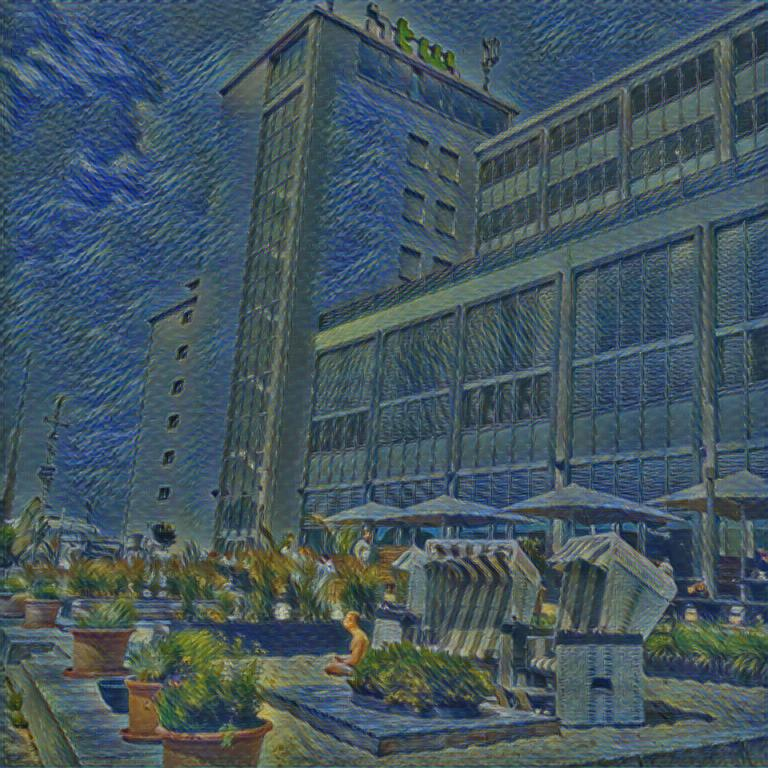
\includegraphics[width=\textwidth]{resources/content/experiments/net8.jpg}
    \end{subfigure}
    \begin{subfigure}[h]{0.15\textwidth}
        \centering
        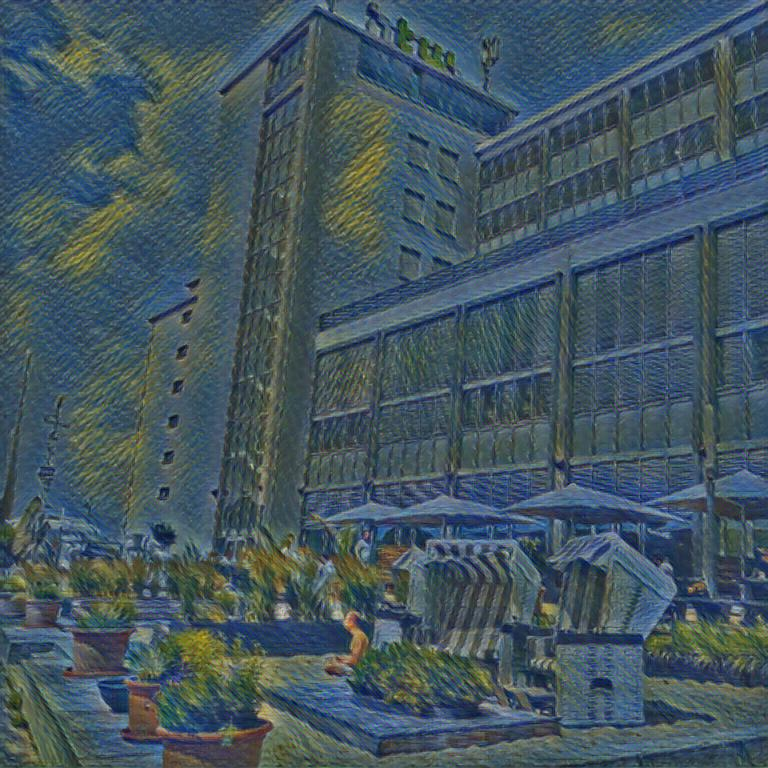
\includegraphics[width=\textwidth]{resources/content/experiments/net9.jpg}
    \end{subfigure}
    \caption{Vergleich der Netzwerke 1 bis 9}
\end{figure}

Daraus kann geschlussfolgert werden, dass sogar das Netzwerk mit den wenigstens lernbaren Parametern, Netzwerk 9, in der Lage ist Stile zu erlernen.
Der arithmische Mittelwert bei der Berechnung von Bildern der Größe 1024 * 768 Pixel mit Netzwerk 9 betrug 0.00414 Sekunden, vgl. \ref{tab:1024x768}. Damit können mehr als 240 Bilder pro Sekunde zu berechnen werden. Somit würde sich die Möglichkeit ergeben komplette Videos in Echtzeit zu berechnen, worauf im Ausblick \ref{sec:video_stylization} eingegangen wird.